%\documentclass[a4paper,landscape, 5pt]{article}
\documentclass[10pt]{article}
\usepackage[a4paper, margin=0.1in, landscape]{geometry}
%\usepackage{graphicx} % Required for inserting images
\usepackage{graphicx}
\usepackage{multicol}
\usepackage{titlesec}
\usepackage{xcolor}
\usepackage{amsfonts}

\setlength{\parindent}{0pt}

%\setlength{\columnsep}{1.5cm}
\setlength{\columnseprule}{0.2pt}

% Adjust spacing before and after sections
\titlespacing\section{0pt}{\parskip}{-\parskip}
% Adjust spacing before and after subsections
\titlespacing\subsection{0pt}{\parskip}{-\parskip}

\begin{document}

\begin{multicols*}{4}

\section{Regression}
\subsection{Terminology}

- Data consists of \textbf{pairs} ($\mathbf{x}_n$, $y_n$), where $y_n$ is the n’th output and $x_n$ is a vector of $D$ inputs. The number of pairs $N$ is the data-size and $D$ is the dimensionality.

- Two goals of regression: \textbf{prediction} and \textbf{interpretation}

- The regression function: $y_{n}\approx f_w(\mathbf{x}_{n})\ \forall n$

- Regression finds correlation not a causal relationship.

- \textbf{Input variables} a.k.a. covariates, independent variables, explanatory variables, exogenous variables, predictors, regressors. 

- \textbf{Output variables} a.k.a. target, label, response, outcome, dependent variable, endogenous variables, measured variable, regressands.

\vspace{4pt}
\hrule
\vspace{4pt}
\subsection{Linear Regression}

- Assumes linear relationship between inputs and output.

- $y_{n}\approx\,f(\mathbf{x}_{n}) :=w_{0}+w_{1}x_{n1}+ ... +w_{D}x_{n D} \\ := \tilde{\bf x}_{n}^{T} \tilde{\bf w}$ contain the additional offset term (\small{a.k.a. bias}).

- Given data we learn the weights $\mathbf{w}$ (\small{a.k.a. estimate or fit the model})

- Overparameterisation $D > N$ eg. univariate linear regression with a single data point $y_{1}\approx w_{0}+w_{1}x_{11}$. This makes the task under-determined (no unique solution).

\vspace{4pt}
\hrule
\vspace{4pt}
\subsection{Loss Functions $\mathcal{L}$}

- A loss function (a.k.a. energy, cost, training objective) quantifies how well the model does (how costly its mistakes are).

- $y \in \mathbb{R} \Rightarrow$ desirable for cost to be symmetric around 0 since $\pm$ errors should be penalized equally.

- Cost function should penalize “large” mistakes and “very large” mistakes similarly to be robust to outliars.

- Mean Squared Error: \\ ${\mathsf{MSE}}(\mathbf{w}):={\frac{1}{N}}\sum_{n=1}^{N}\left[y_{n}-f_{\mathrm{w}}(\mathbf{x}_{n})\right]^{2}$ \\ not robust to outliars.

- Mean Absolute Error: \\ ${\mathsf{MAE}}(\mathbf{w}):={\frac{1}{N}}\sum_{n=1}^{N}|y_{n}-f_{\mathrm{w}}(\mathbf{x}_{n})|$

- Convexity: a function is convex iff a line segment between two points on the function’s graph always lies above the function.

- Convexity: a function $h(\mathbf{u}), \mathbf{u} \in \mathbb{R}^D$ is convex if $\forall \ \mathbf{u}, \mathbf{v} \in \mathbb{R}^D, 0 \leq \lambda \leq  1$: \\ $h(\lambda\mathbf{u}+(1-\lambda)\mathbf{v}) \ \textcolor[RGB]{255,0,0}{\leq} \ \lambda h(\mathbf{u})+(1-\lambda)h(\mathbf{v})$ \\Stirctly convex if $\textcolor[RGB]{255,0,0}{\leq} \Rightarrow \textcolor[RGB]{255,0,0}{<}$ 

- Convexity, a desired computational property:
A strictly convex function has a unique global minimum $\mathbf{w^{*}}$. For convex functions, every local minimum is a global minimum.

- Sums of convex functions are also convex $\Rightarrow$ MSE combined with a linear model is convex in $\mathbf{w}$.

- Proof of convexity for MAE:

\scalebox{0.7}{
$\begin{array}{l}
    {\mathsf{MAE}(\mathbf{w}) := \frac{1}{N} \sum_{n=1}^{N} \mathcal{L}_n(\mathbf{w}), \mathcal{L}_n(\mathbf{w})=|y_{n}-f_{\mathrm{w}}(\mathbf{x}_{n})|} 
    \\ 
    {\mathcal{L}_n(\lambda w_1 + (1-\lambda)w_2) \leq \lambda \mathcal{L}_n(w_1)+(1-\lambda)\mathcal{L}_n(w_2)} 
    \\ 
    {| y_n-x_n^{T}(\lambda w_1 + (1-\lambda)w_2)| \leq \lambda |{y_n-x_n^{T}w_1}| + (1-\lambda)|{y_n-x_n^{T}w_2}|}
    \\
    {(1-\lambda) \geq 0 \Rightarrow (1-\lambda)|{y_n-x_n^{T}w_2}|=|(1-\lambda)y_{n}-(1-\lambda)x_{n}^{T}w_2|}
    \\
    {a=\lambda y_{n}-\lambda x_{n}^{T}w_{1}, b=(1-\lambda)y_{n}-(1-\lambda)x_{n}^{T}w_{2}}
    \\
    {a+b=y_{n}-x_{n}^{T}(\lambda w_{1}+(1-\lambda)w_{2})}
    \\
    {|a + b| \leq |a| + |b| \Rightarrow \mathcal{L}_n(\mathbf{w}) \ \mathsf{convex}\Rightarrow \mathsf{MAE}(\mathbf{w}) \ \mathsf{convex}}
\end{array}$
}

- Huber loss: \\
${\cal H}u b e r(e):=\left\{\begin{array}{l l}{{\frac{1}{2}e^{2}}}&{{,\mathrm{if}\ |e|\leq\delta}}\\ {{\delta|e|-\frac{1}{2}\delta^{2}}}&{{,\mathrm{if}\ |e|>\delta}}\end{array}\right.$ convex, differentiable, and robust to outliers but setting $\delta$ is not easy.

- Tukey’s bisquare loss: \\
$\frac{\partial\mathcal{L}}{\partial e}:=\left\{\begin{array}{l l}{{e\{1-e^{2}/\delta^{2}\}^{2}}}&{{,\mathrm{if}\,\,|e|\leq\delta}}\\ {{0}}&{{,\mathrm{if} \ |e| > \delta}}\end{array}\right.$ non-convex, but robust to outliers.

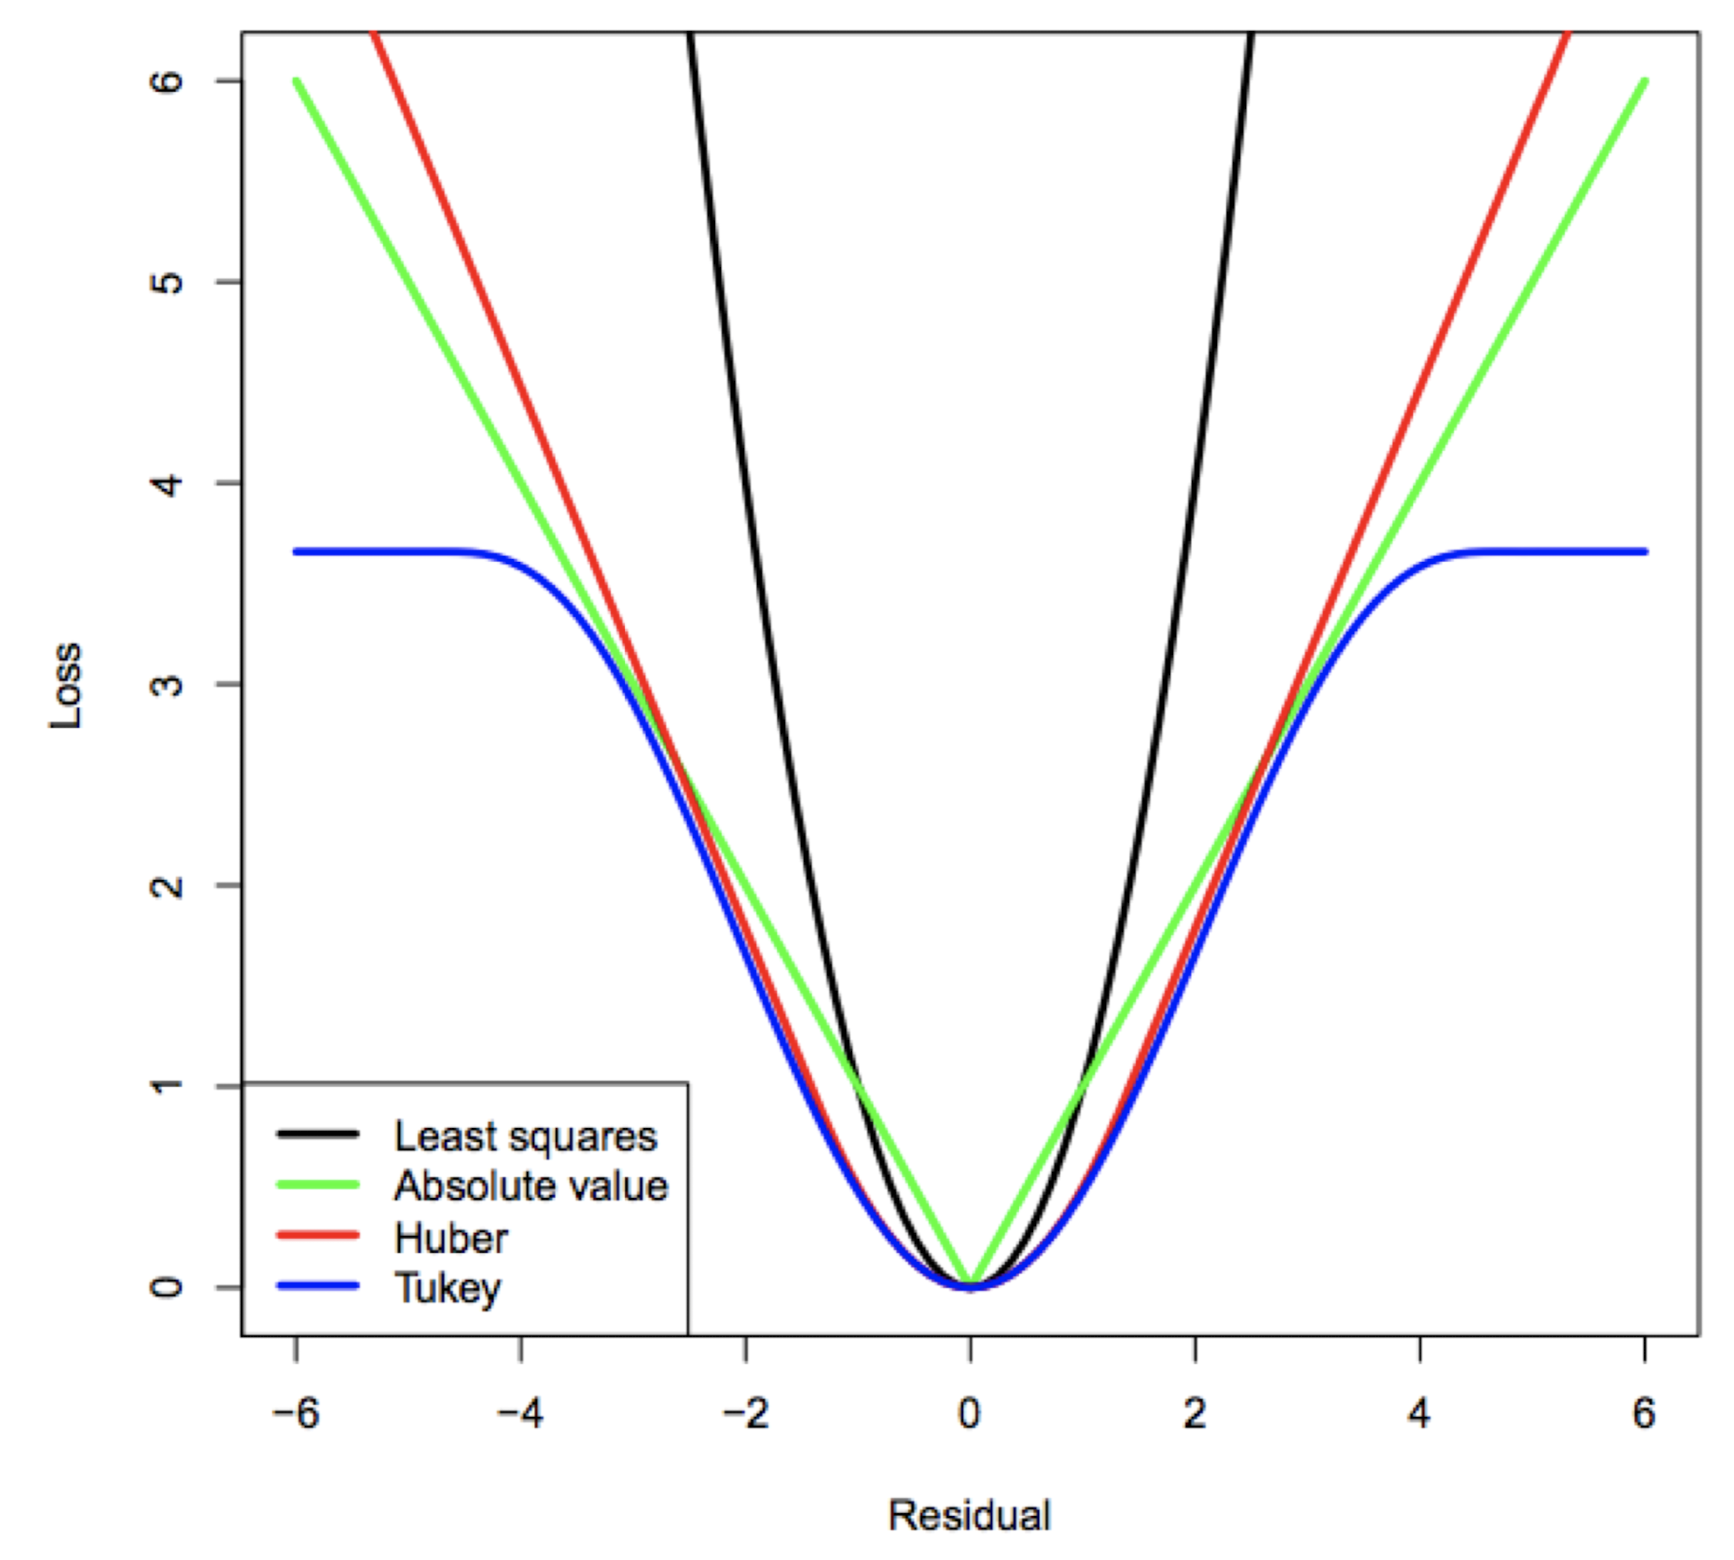
\includegraphics[width=\linewidth]{loss_functions.png}

\vspace{4pt}
\hrule
\vspace{4pt}
\section{Optimisation}

- Given $\mathcal{L}(\mathbf{w})$ we want $\mathbf{w^*} \in \mathbb{R}^D$ which minimises the cost: $\min_\mathbf{w} \mathcal{L}(\mathbf{w}) \rightarrow$ formulated as an optimisation problem

- Local minimum $\mathbf{w^*} \Rightarrow \exists \epsilon > 0$ s.t. \\
$\mathcal{L}(\mathbf{w^*}) \leq \mathcal{L}(\mathbf{w}) \ \forall \mathbf{w} \ \mathrm{with} \ \Vert \mathbf{w}-\mathbf{w^*} \Vert < \epsilon$

- Global minimum $\mathbf{w^*}$,
$\mathcal{L}(\mathbf{w^*}) \leq \mathcal{L}(\mathbf{w}) \ \forall \mathbf{w} \in \mathbb{R}^D$

\subsection{Smooth Optimisation}



\newpage
\section{{\textcolor[RGB]{255,0,0}{This is RGB red text.}}}

For $x \in[r_{i-1},r_{i}]$ \\
$r(x)={\tilde{a}}_{1}x+{\tilde{b}}_{1}+\sum_{j=2}^{m}{\tilde{a}}_{j}(x-{\tilde{b}}_{j})_{+}$

\hrulefill

$\begin{array}{l}{{\mathsf{For}\;x\in[r_{i-1},r_{i}]}}\\ {{r(x)={\tilde{a}}_{1}x+{\tilde{b}}_{1}+\sum_{j=2}^{m}{\tilde{a}}_{j}(x-{\tilde{b}}_{j})_{+}}}\end{array}$\\
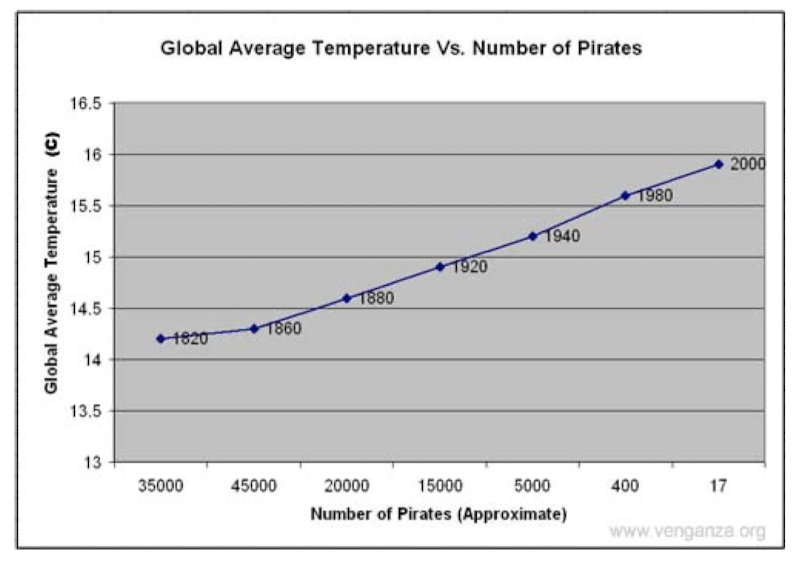
\includegraphics[width=\linewidth]{test_image}

Once upon a time in the whimsical town of Serendipity Springs, there lived a peculiar inventor named Professor Quixotic. Known for his wild ideas and even wilder inventions, the professor spent his days tinkering away in his eccentric laboratory.

\noindent\dotfill

One day, while experimenting with a contraption designed to turn laughter into energy, Professor Quixotic accidentally created a portal to a parallel universe. As the portal crackled with energy, it sucked the professor and his loyal robotic sidekick, Gizmo, into a world where everything was upside down.

In this topsy-turvy land, gravity worked in reverse, causing the duo to float above the ground. Trees grew with their roots in the air, and people walked on the ceilings of their homes. It was a place of perpetual confusion and constant laughter.

As Professor Quixotic and Gizmo explored this strange realm, they encountered a group of upside-down creatures called the Giggleglides. These whimsical beings thrived on laughter and had the power to make anything levitate with a simple joke.

Realizing the potential of this upside-down world, Professor Quixotic teamed up with the Giggleglides to create a laughter-powered flying machine. With the combined ingenuity of the professor and the Giggleglides' comedic talents, they built the most extraordinary aircraft the upside-down world had ever seen.

The laughter-powered flying machine soared through the topsy-turvy skies, spreading joy and amusement wherever it went. The upside-down inhabitants were thrilled to have a new form of transportation that brought them even closer to the upside-down stars.

Eventually, Professor Quixotic and Gizmo found another portal, one that led them back to Serendipity Springs. The laughter-powered flying machine became a symbol of the magical adventure, and the town embraced the upside-down spirit with open arms.

And so, the town of Serendipity Springs became a place where laughter powered not only inventions but also the hearts of its inhabitants. Professor Quixotic continued his quirky experiments, inspired by the upside-down world, and the memory of the laughter-filled adventure remained etched in the hearts of all who experienced it.


\end{multicols*}

\end{document}
